% Estado de la extracción núcleo por celda (fig:horizontal). Fuente:
% ../tablas/horizontal_revision.csv (columna estado_extraccion), comprobación del 2026-11-07.
% Recuentos a mano: completa 8, incompleta 4, otro protocolo 6, sin archivo 6; total 24.
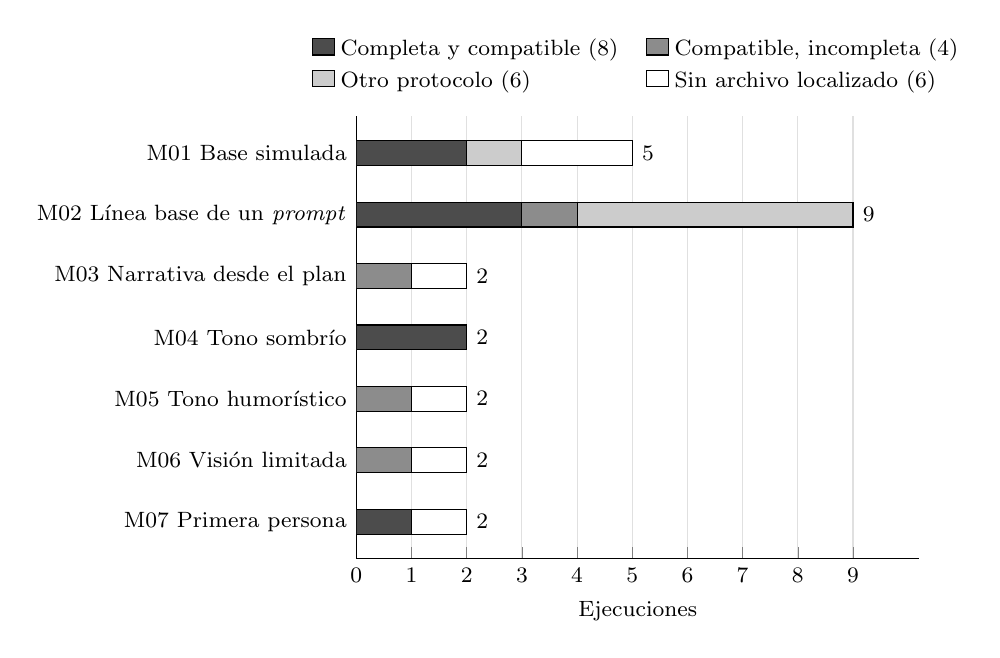
\begin{tikzpicture}
  \begin{axis}[
      xbar stacked,
      width=0.72\textwidth,
      height=7.2cm,
      bar width=9pt,
      font=\footnotesize,
      xmin=0, xmax=10.2,
      xtick={0,1,...,9},
      xlabel={Ejecuciones},
      ytick={1,...,7},
      yticklabels={
        M01 Base simulada,
        M02 Línea base de un \textit{prompt},
        M03 Narrativa desde el plan,
        M04 Tono sombrío,
        M05 Tono humorístico,
        M06 Visión limitada,
        M07 Primera persona},
      y dir=reverse,
      ymin=0.4, ymax=7.6,
      axis x line*=bottom,
      axis y line*=left,
      xmajorgrids,
      major grid style={draw=black!12},
      tick style={draw=black!50},
      legend style={at={(0.5,1.03)}, anchor=south, legend columns=2, draw=none,
        font=\footnotesize, /tikz/every even column/.append style={column sep=8pt}},
      legend cell align=left,
    ]
    \addplot[fill=black!70, draw=black] coordinates
      {(2,1) (3,2) (0,3) (2,4) (0,5) (0,6) (1,7)};
    \addplot[fill=black!45, draw=black] coordinates
      {(0,1) (1,2) (1,3) (0,4) (1,5) (1,6) (0,7)};
    \addplot[fill=black!20, draw=black] coordinates
      {(1,1) (5,2) (0,3) (0,4) (0,5) (0,6) (0,7)};
    \addplot[fill=white, draw=black] coordinates
      {(2,1) (0,2) (1,3) (0,4) (1,5) (1,6) (1,7)};
    \legend{Completa y compatible (8), {Compatible, incompleta (4)},
      Otro protocolo (6), Sin archivo localizado (6)}
    % Total de ejecuciones de cada celda, al final de su barra.
    \node[anchor=west] at (axis cs:5,1) {5};
    \node[anchor=west] at (axis cs:9,2) {9};
    \node[anchor=west] at (axis cs:2,3) {2};
    \node[anchor=west] at (axis cs:2,4) {2};
    \node[anchor=west] at (axis cs:2,5) {2};
    \node[anchor=west] at (axis cs:2,6) {2};
    \node[anchor=west] at (axis cs:2,7) {2};
  \end{axis}
\end{tikzpicture}
